% Thesis template, taken from CVPR 2022 paper template.
% CVPR 2022 Paper Template
% based on the CVPR template provided by Ming-Ming Cheng (https://github.com/MCG-NKU/CVPR_Template)
% modified and extended by Stefan Roth (stefan.roth@NOSPAMtu-darmstadt.de)

\documentclass[10pt,twocolumn,letterpaper]{article}

%%%%%%%%% PAPER TYPE  - PLEASE UPDATE FOR FINAL VERSION
%\usepackage[review]{sarmata}      % To produce the REVIEW version
\usepackage{sarmata}              % To produce the CAMERA-READY version
%\usepackage[pagenumbers]{cvpr} % To force page numbers, e.g. for an arXiv version

% Include other packages here, before hyperref.

\usepackage{multirow}
\usepackage{graphicx}
\usepackage{float}
\usepackage{amsmath}
\usepackage{amssymb}
\usepackage{booktabs}
\usepackage[pagebackref,breaklinks,colorlinks]{hyperref}
\usepackage[none]{hyphenat}
% Support for easy cross-referencing
\usepackage[capitalize]{cleveref}
\crefname{section}{Sec.}{Secs.}
\Crefname{section}{Section}{Sections}
\Crefname{table}{Table}{Tables}
\crefname{table}{Tab.}{Tabs.}


\begin{document}

\begin{titlepage}
    \begin{center}
        % Logos
        
\includegraphics[width=0.3\textwidth]{hhu_logo.png} \hfill \\[1cm]

        {\Large\textsc{Heinrich-Heine-Universität D\"usseldorf}}\\[3cm]
        {\Large\textbf{Bachelor Thesis}}\\[1cm]

        {\Huge\textbf{Implementierung und Evaluation der Reinforcement-Learning-Methoden Self-Play und Liga-Training in der MicroRTS-Umgebung}}\\[2cm]

        {\Large\textbf{{Name!!!!!!!!!!!!!!!!!!!!!!!!!!!!!!!!!!!!!!!!!!!!!!!!!!!!!!!!!!!!!!!!!!!!!!!!!!!!!!}}}\\[2cm]

        \vfill
        % Details
        \begin{tabbing}
            \hspace{4cm} \= \hspace{8cm} \= \\ % Tab stops
            Degree: \> B.Sc. Computer Science \\
            Supervisor: \> Professor Dr. Paul Swoboda \\
            Co-Supervisor: \> Dr. Peter Arndt \\
            Faculty: \> Mathematisch-Naturwissenschaftliche Fakultät \\
        \end{tabbing}

        \vfill % Vertical space

        {\large XXXXXXXXXXX}
    \end{center}
\end{titlepage}

%%%%%%%%% ABSTRACT
\begin{abstract}
    % (???) Wir oder ich?
    This thesis improves an existing agent for the real-time strategy game (RTS) MicroRTS.
    RTS games are considered a challenging domain for Deep Reinforcement Learning (DRL), since agents must deal with large combinatorial action spaces, simultaneous decisions, as well as delayed and often sparse rewards.
    As a baseline method, we use Proximal Policy Optimization (PPO).
    In many DRL training setups, such as pure PPO, one reaches a point at which the agent cannot be trained further efficiently using PPO alone, because there are not enough strong opponents to train against or because the available opponents are not diverse enough to develop a robust policy.
    An obvious and simple countermeasure is Self-Play (SP) however, in practice it can be unstable and lead to overfitting or cyclical strategies, which can reduce performance against external opponents.


    League Training (LT) stabilizes SP by building a population of agents across different training stages and roles. The training agent is then deliberately matched against diverse opponents. Among others, against specialized agents that were trained to exploit weaknesses of the current policy. We evaluate the resulting agents in matches against various opponent types and compare LT with pure SP as well as with our initial agent. Our results show that LT increases the robustness and generalization capability of the agent against different opponents.

\end{abstract}


\tableofcontents
\newpage

%%%%%%%%% BODY TEXT´
\section{Introduction}
\label{sec:Introduction}

Reinforcement Learning (RL) has established itself in recent years as a powerful approach for developing agents in complex environments. 
Game environments such as RTS games pose a particular challenge in this regard, with large action spaces, long-term planning, and simultaneous decisions. However, they also provide clearly defined state spaces, reward structures, and repeatable experiments, which makes them an ideal and challenging test environment for researching RL methods.

\paragraph{MicroRTS}
MicroRTS is a simplified version of RTS games that was developed specifically for research \cite{huang2021gym}. 
It is discrete and reduces the visual and mechanical complexity of large commercial RTS games, such as StarCraft II. 
At the same time, it retains the core difficulties, for example resource management, unit production, combat mechanics, and tactical positioning. 
MicroRTS is therefore suitable for the systematic investigation of learning methods. MicroRTS also contains numerous training challenges, such as large combinatorial action spaces, delayed rewards, multi-agent interactions, and it also requires robust strategies against different opponents. 
For example, the agent must decide early on whether it wants to play aggressively or defensively against the current opponent, which affects the overall game strategy and requires long-term planning.

\paragraph{Self-Play-Based Approaches.}
A central problem in RL is generalization across different opponents and strategies: agents often learn strategies that are strongly tailored to the training opponent or a specific game situation. 
This leads to overfitting and limited robustness. 
SP, Fictitious Self-Play (FSP), and LT are approaches that address this problem. 
In SP, the agent trains by playing against itself, which leads to a continuous learning process that does not require additional diverse or strong opponents. 
However, training is often unstable because of cyclical learning.
% Ein Beispiel: Spielt der Agentzustand B gut gegen A, C gut gegen B und A gut gegen C, könnte der Agent in einem Zyklus gefangen sein, in dem er immer nur den Agentenzustand wieder erlernt, der gegen sich selbst gut ist, aber nicht gegen andere Gegner.

\paragraph{league training (LT).}
To reduce the instabilities of pure SP, the agent in FSP is not trained against the current agent but against previous versions of itself, which prevents cyclical learning \cite{heinrich2015fsp}. % and converges to the Nash equilibrium in two-player zero-sum games 
LT extends FSP by training the agent against historical opponents from a league that consists of different agent types, for example policy snapshots from earlier training stages as well as specialized agents \cite{vinyals2019alphastar}.
The goal is to stabilize the learning environment, in which agents compete against a broad spectrum of strategies and thereby become more robust.

\paragraph{Thesis Outline:}
Despite the theoretical advantages, the practical implementation of LT in complex environments such as MicroRTS is associated with significant challenges, that need to be addressed. 
These include:
\begin{itemize}
    %TODO: füge weitere hinzu
    \item the efficient management and selection of opponents for training the Main Agent and for the specialized agents,
    \item stabilizing the training process under non-constant opponent distributions,
    \item dealing with large action spaces and sparse or delayed rewards, and
%\item assessing the actual generalization capability of the trained agents.
\end{itemize}
In addition, we will compare and evaluate the Results emperically. 
In particular, we will analyze the learning curve, strategic diversity, and robustness for the different training approaches.

\paragraph{Training the Base Agent:}
The base agent used in this project is trained in a three-stage procedure that combines BC and BC fine-tuning (BC-FT), followed by fine-tuning with PPO:
The two BC phases enable the agent to quickly learn a competent base strategy by imitating expert behavior \cite{torabi2018behavioral}. 
This training approach reduces the initial, often inefficient exploration in DRL \cite{torabi2018behavioral}. 
Learning from scratch with DRL methods such as PPO can be very time-consuming \cite{martin2021beclone}. 
PPO is a well-known on-policy policy optimization method that clips the policy update size to stabilize policy updates \cite{schulman2017ppo}.
PPO further improves the performance of the BC agent through exploration and adaptation to the environment, allowing the agent to adapt and generalize beyond the expert strategies \cite{martin2021beclone}. 
This two-stage approach, in which a policy pre-trained with BC is refined by a DRL algorithm, has proven effective in reducing training time and improving overall performance compared to a pure DRL approach \cite{martin2021beclone}.



\section{Related Work}
\label{sec:related-work}
% TODO: \textbf und \paragraph sehen sehr ähnlich aus. (\paragraph sollte unter \textbf liegen)
\noindent\textbf{Game Playing Agents in MicroRTS}
The (unpublished) bachelor’s thesis by M. Huft that underlies this work develops a competitive agent for MicroRTS and evaluates the hybrid training pipeline consisting of BC, BC-FT, and PPO for the base agent from the introduction \cite{huft2023microrts}.

\paragraph{Results and Limitations.}
The results show a clear performance increase across all three training phases (Table~\ref{tab:win rates_all}): BC mainly learns basic game mechanics, while BC-FT improves generalization against multiple bots. Finally, PPO achieves high win rates against many of the built-in bots \cite{huft2023microrts}.
There still are agents in the results against which the base agent does not perform well. 
The thesis also identifies limitations, in particular the focus on a single map and the limited opponent diversity, and proposes extensions using self-play or league mechanisms. 
Exactly this proposal is taken up by the present work by extending the existing base agent and the initial code with SP and LT. 
The opponents against which the evaluation is conducted include the MicroRTS built-in bots (RandomBiasedAI, WorkerRushAI, LightRushAI, and CoacAI).
\begin{table}[ht]
\centering
\caption{Winrates (\%) for BC, BC-FT, and PPO reported in \cite{huft2023microrts}.}
\label{tab:win rates_all}
\begin{tabular}{lccc}
\hline
\textbf{Bot} & \textbf{BC} & \textbf{BC-FT} & \textbf{PPO} \\
\hline
WorkerRushAI     & 3 & 50 & 99 \\
PassiveAI        & 98& 100& 100 \\
LightRushAI      & 22 & 93 & 99 \\
CoacAI           & 0 & 8 & 96 \\
Mayari           & 0 & 5 & 95 \\
RandomAI         & 52 & 95 & 99\\
RandomBiasedAI   & 18 & 68 & 86\\
rojo             & 0 & 34& 84 \\
mixedBot         & 4 & 44 & 59 \\
izanagi          & 0& 62& 61\\
tiamat           & 11 & 78& 84 \\
droplet          & 0& 31& 59\\
guidedRojoA3N    & 4 & 42& 75 \\
naiveMCTS        & 0 & 5& 3 \\
\hline
\end{tabular}
\end{table}
\vspace{10pt}

\noindent\textbf{MicroRTS-Py (Gym-$\mu$RTS)}
Huang et al. provide an efficient Gym-compatible interface for our environment MicroRTS \cite{Ontanon2013CombinatorialBandit} with \emph{Gym-$\mu$RTS} / \emph{MicroRTS-Py} \cite{huang2021gym}.
MicroRTS-Py is an established and widely used DRL baseline that enables the investigation of DRL approaches in full real-time strategy game scenarios without requiring extensive technical infrastructure such as high-performance computing clusters \cite{huang2021gym}.

\paragraph{Proximal Policy Optimization (PPO) training.}
The \emph{openai/baselines} \cite{baselines} implementation of PPO was adapted in order to fit MicroRTS-Py. We use a large part of this implementation in LT \cite{huang2021gym}. 
It was also previously used in the PPO training phases of the base agent \cite{huft2023microrts}.
On top of openai/baselines, \emph{invalid action masking} and suitable action/observation representations (e.g., GridNet \cite{pmlr-v97-han19a}) as well as architectural choices (such as IMPALA-CNN-a deep convolutional neural network structure with residual blocks for processing grid-based state representations in RL) \cite{espeholt2018impala} were added \cite{huang2021gym}. 
In a modified form, these are still used in the LT code.

\paragraph{GridNet.}
Huang et al. considered using \emph{GridNet} or \emph{Unit Action Simulation} (UAS) instead of GridNet. 
UAS iterates over all units at each step and returns the possible actions for each unit, which substantially reduces the action space. 
GridNet, in contrast, predicts an action for each cell on the map. This means that GridNet executes its large action space in a single step, but this also simplefies the training \cite{huang2021gym, pmlr-v97-han19a}.
Against the built-in bots of MicroRTS, which are based on heuristic rules, the PPO implementation with invalid action masking and IMPALA-CNN achieves an average win rate of 91\% with UAS and 84\% with GridNet. Ultimately, the decision was made to focus on GridNet, since its complexity is lower, and it facilitates compatibility with SP (and LT) \cite{huang2021gym}.
SP was also evaluated in the work. However, there was a bug in the code that likely strongly affected the results for SP \cite{goodfriend2024raisocketai}.
\vspace{10pt}

\noindent\textbf{RAISocketAI}
In 2023 RAISocketAI was the first DRL agent which won the IEEE MicroRTS Competition. RAISocketAI includes a re-implementation of MicroRTS-Py, which is used in our code. 
Among other things, data generation via replays is an important basis for BC \cite{huft2023microrts}, and a bug in the old implementation was fixed that marked non-owned resources as owned resources when the agent is player 2. 
According to Goodfriend, this likely caused SP in the previous MicroRTS-Py implementation to yield no improvements, The RAISocketAI implementation of FSP achieved an average win rate of 91\% against the same MicroRTS built-in bots as in MicroRTS-Py, which is significantly higher than 84\% in the previous implementation. 
However, FSP achieved only a 20\% win rate against CoacAI, whereas the best previous implementations were almost always able to defeat CoacAI. 
With fine-tuning on CoacAI and Mayari, the average win rate against the built-in bots was increased to 98\% \cite{goodfriend2024raisocketai}.
LT was not implemented or evaluated in the work.
\vspace{10pt}

\noindent\textbf{BeClone}
\emph{BeClone} demonstrated the effectiveness of BC with DRL fine-tuning in MicroRTS-Py using a two-phase training strategy for RTS agents: first, an initial policy is learned from experts via BC, and subsequently an RL fine-tuning is performed using \emph{Advantage Actor-Critic} (A2C) \cite{martin2021beclone}.
\vspace{10pt}

\noindent\textbf{AlphaStar}
Alphastar is a DRL agent for the complex RTS game StarCraft II, which was developed by DeepMind \cite{vinyals2019alphastar}.
It demonstrates that LT can decisively contribute to robustness in complex RTS domains. 
The agent in AlphaStar was pre-trained with \emph{imitation learning} from human replays. 

\paragraph{Pre-League Training.}
In this thesis, we replace imitation learning with the BC phases and the PPO phase. 
Similar to AlphaStar our agent was further trained in a league of different agent types (Main Agent, Main Exploiters, League Exploiters, and historical snapshots (\emph{historical agents})) to reduce overfitting and forgetting and to promote diversity. 

\paragraph{League Composition and Training.}
As in AlphaStar, in this thesis Main Exploiters are trained by training the base agent against all historical versions of the Main Agenten in the league, in order to identify and exploit weaknesses.
At the same time, League Exploiters train against all historical agents.
The Main Agent trains with \emph{Prioritized fictitious self-play} PFSP against historical versions of itself, Main Exploiters, and League Exploiters.
The prioritization of the historical opponents is computed based on the Main Agent’s win rate against the respective historical agents.
In this thesis, the prioritization formula was adjusted to better fit the MicroRTS environment.
An exploiter is added to the league as a historical agent only when it shows a high win rate against all opponents or when a predefined step limit is reached \cite{vinyals2019alphastar}. 

\paragraph{Differences from AlphaStar.}
Although MicroRTS and StarCraft II substantially differ in complexity and representation, AlphaStar is an established reference design for stabilizing and generalizing SP through league-based matchmaking mechanisms and the inclusion of specialized exploiters \cite{vinyals2019alphastar}.
AlphaStar performs policy updates using an \emph{actor–critic method} with an off-policy correction mechanism called \emph{V-trace} \cite{espeholt2018impala, vinyals2019alphastar}.
This approach is better suited for LT than PPO due to its robustness to off-policy data and its typically better scalability in large distributed setups.
However, the implementation of PPO in MicroRTS-Py is significantly simpler and faster to realize, which is why PPO is a practical choice for implementing LT \cite{vinyals2019alphastar}.
In addition, AlphaStar uses TD($\lambda$) \cite{suttonbarto1998rl} for value estimation value-function estimation.


\section{Methods}
\label{sec:Methods}
\subsection{MicroRTS-environment}
\label{sec:MicroRTS-environment}
MicroRTS is a two-player zero-sum game that is played on a two-dimensional grid (the map).
Different units can be located on each cell of this map, and players can execute actions to move/train/attack units and to collect resources.
The different units are:

\newcommand{\uniticon}[2][1.6em]{%
  \raisebox{-0.25\height}{\includegraphics[height=#1]{#2}}%
}

\paragraph{Unit Types.}
\begin{itemize}
\item \textbf{Base:} \uniticon{images/Base.png} The Base can store resources and train Workers. It is very important, since it is the only way to store resources. (Cost (in resources): 10, hit points (hp): 10)
\item \textbf{Resources:} \uniticon{images/Resource.png} There is only one type of resource. It can be stored by Workers in the Base. (Number of resources in a cell: depends on the map in our case 25)
\item \textbf{Worker:} \uniticon{images/Worker.png} Workers can collect resources and build Barracks. (Cost: 1, hp: 1, attack strength (at): 1)
\item \textbf{Barracks:} \uniticon{images/Barracks.png} Barracks can train Light, Heavy, and Ranged units. (Cost: 5, hp: 4)
\item \textbf{Light:} \uniticon{images/Light.png} Light units can move quickly, are trained quickly, and cost little. (Cost: 2, hp: 4, at: 2)
\item \textbf{Heavy:} \uniticon{images/Heavy.png} Heavy units can move slowly are trained slowly and cost a lot, but have high at and hp. (Cost: 3, hp: 8, at: 4)
\item \textbf{Ranged:} \uniticon{images/Ranged.png} Ranged units have an attack range of 3 cells. (Cost: 2, hp: 1, at: 1)
\end{itemize}
Worker, Light, Heavy, and Ranged units can move one cell in one of four directions.
Units of player 1 are displayed with a blue outline, whereas units of player 2 are outlined in red.
Movement is visualized with a gray line, attacking with a red line, and gathering with a green line.

\paragraph{Game Setup.}
Most games are decided within 2000 steps. Therefore, the maximum number of steps is set to 2000.
The experiments in this thesis were conducted using the RAISocketAI re-implementation of MicroRTS and the map \texttt{basesWorkers16x16A}, which is shown in Figure~\ref{Figure 1}.
This symmetric map starts each player with one Base, five resources, two Workers, and 50 resources near the Base. \textbf{\cite{goodfriend2024raisocketai}}

\begin{figure}[H]
    \centering
    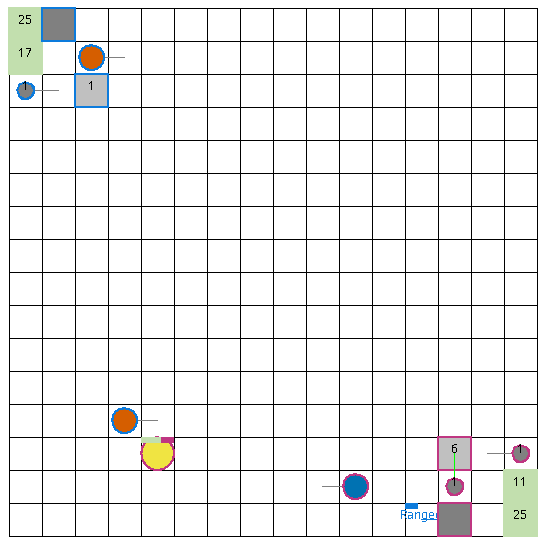
\includegraphics[width=1\linewidth]{images/16x16.png}
    \caption{Screenshot \texttt{basesWorkers16x16A} map \cite{huft2023microrts}.}
    \label{Figure 1}
\end{figure}

\paragraph{Action Space.}
The action space used in this thesis is implemented using the combination of GridNet and invalid action masking \cite{huang2021gym}.
GridNet produces a unit action (an action for one specific cell) for each cell of the map, regardless of whether a unit is located on the cell and whether the action is valid \cite{pmlr-v97-han19a}.
Building on this, invalid action masking is used to mask invalid actions, thereby also masking actions empty cells \cite{huang2021gym}.
The \emph{unit action space} is defined as an 8-dimensional vector per cell:
\[
(\text{pos}, \text{type}, d_{\text{move}}, d_{\text{harvest}}, d_{\text{return}}, d_{\text{produce}}, \text{pType}, \text{relPos})
\]
The components of the unit-action vector are defined as follows:
\begin{itemize}
\item \textbf{pos:} Linearized index of the cell in the grid (i.e., the grid represented in a one-dimensional space; e.g., for a $16\times 16$ grid: range: [0, 255]).
\item \textbf{type:} Action type (range: [0, 5], 0: Nop, 1: Move, 2 Harvest, 3: Return, 4: Produce, 5: Attack).
\item \textbf{$d_{\text{move}}, d_{\text{harvest}}, d_{\text{return}}, d_{\text{produce}}$:} Directions (range: [0, 3], 0: North, 1: East, 2: South, 3: West) for the respective actions.
\item \textbf{pType:} Type of the unit to be produced. (range: [0, 6], 0: Resource, 1: Base, 2: Barracks, 3: Worker, 4: Light, 5: Heavy, 6: Ranged).
\item \textbf{relPos:} Relative attack position. (range: [0, 48]).
\end{itemize}
For our agent, the unit action space (without the position dimension) is linearized and represented using one-hot encoding.
The position is implicitly encoded by the linear grid indexing of the GridNet output \cite{huang2021gym}.
Given a map of size $h \times w$, the action space has shape $h \times w \times 78$.
For our $16 \times 16$ map, the action space per environment in the GridNet representation would therefore contain $16 \times 16 \times 78 = 19968$ actions. However, many of them can be invalid and are masked by invalid action masking \cite{huang2021gym}.
Afterward the position is incorporated before masking the actions, otherwise the masking would remove the structure of the Action-Space, which would remove the implicit encoding for the position.
Depending on the action type, only parts of the action vector are relevant (e.g., if the action type is \texttt{Move}, then only the components \texttt{pos}, \texttt{type}, and \texttt{$d_{\text{move}}$} are relevant (the other components are ignored)).


\paragraph{Observation Space.}
Observations are represented as a grid of shape $h \times w \times c$ per environment, where $h$ and $w$ are the height and width of the map, and $c$ is the number of encoded features of each cell in the game state (e.g., unit types, hit points, move direction, etc.) \cite{huang2021gym}.
The screenshot of the map basesWorkers16x16A \ref{Figure 1} visualizes the observation space, without any additional information.


\subsection{Training Pipeline}
The training pipeline extended in this thesis consists of four phases: BC, BC-FT, PPO, and LT (or FSP/SP).
The first three phases were already implemented in the previous work \cite{huft2023microrts} and are only briefly described here.
In BC/BC-FT, demonstrations from experts (here, the built-in bots CoacAI and Mayari) are used to train an initial policy to learn basic game mechanics/strategies \cite{huft2023microrts}.
\begin{itemize}
    \item The BC phases reduces the initial, often inefficient exploration in DRL methodes such as PPO, which can be very time-consuming when trained from scratch \cite{torabi2018behavioral, martin2021beclone}.
    % Insbesondere in MicroRTS, wo die Belohnungen anfänglich besonders spärlich und verzögert sein können, durch die hohe kompetenz der Gegner, die der Agent zu Beginn des Trainings hat, und durch die Komplexität der Umgebung, kann ein reines DRL-Training ohne Vortraining sehr ineffizient sein \cite{martin2021beclone}.
    \item The third phase improves the generalization and performance of the agent through additional exploration beyond expert demonstrations \cite{martin2021beclone}.
    PPO is an on-policy policy optimization method that constrains the size of policy updates in order to achieve stable training \cite{schulman2017ppo}.
    % Typischerweise wird PPO als Actor-Critic-Verfahren dargestellt, in dem der Actor die Policy repräsentiert und der Critic die Value-Funktion schätzt \cite{schulman2017ppo}.
    % Aus den Trajectories, die in einem Rollout gesammelt wurden werden Advantage-Schätzungen berechnet.
    % Diese werden als Signal für die Policy-Updates verwendet.
    % In der Implementierung wird die Loss funktion, die aus der negativen PPO-Zielfunktion besteht mit einem Gradientenabstieg minimiert, was äquivalent zur Maximierung der PPO-Zielfunktion ist \cite{schulman2017ppo}.
    % Die PPO-Zielfunktion besteht aus drei zentralen Termen: einem Policy-Term, der die erwartete Belohnung unter der Begrenzung der Policy-Updates durch die Clipping-Funktion maximiert, einem Value-Term für die Minimierung des Fehlers in der Value-Schätzung und einen Entropie-Term, der durch Maximierung der Aktionsentropie die Exploration fördert \cite{schulman2017ppo}. 
    
    % TODO: vielleicht nur LT ansprechen, wenn ich nicht mehr genug Zeit habe, um FSP zu evaluieren.
    \item Using SP/FSP/LT, we aim to further generalize the base agent by training PPO not only against the built-in bots of MicroRTS (against which the base agent already achieves a high win rate), but also against opponents of equal strength or stronger.
    However, many opponents at this level of performance are not suitable for training, since they are very slow and thus slow down the collection of rollouts for PPO.
    In addition, the agent’s generalization capability improves only to a limited extent when training against only a few new opponents, if the training environment does not provide sufficient opponent diversity.
    SP/FSP/LT address both problems by providing numerous opponents that continue to evolve over the course of training and achieve a high win rate against historical versions of the current agent.
\end{itemize}

\subsection{self-play (SP)}
In SP, the agent trains against its own current version, which leads to a continuous learning process with a co-evolving opponent \cite{doi:10.1126/science.aar6404}.

\paragraph{Implementation.} 
To implement SP in the MicroRTS-Py reimplementation Huang et al. implemented the environment to output the observations (obs) and rewards for both players, which allows the agent to train against itself by simply using the same policy for both players \cite{huang2021gym}.
In RAISocketAI, that approach was improved and fixed \cite{goodfriend2024raisocketai}.
In this Thesis, the same approach with some adustments is used to implement SP, which is also used as a basis for FSP and LT.

\paragraph{Problems:}
\begin{itemize}
    \item The training is often unstable because of cyclical learning.
    For \textbf{example},  if policy B performs well against A, C performs well against B, and A performs well against C, the agent may be trapped in a cycle in which it repeatedly relearns only the policy that performs well against itself, but not against other opponents \cite{vinyals2019alphastar}.
    \item A big problem in the SP training setup is that the agent has to learn to play as player 2 as well as player 1, which complicates the training and can lead to a slow learning process \cite{huang2021gym}.
    The biggest difference between player 1 and player 2 is that player 1 starts at the top left of the map, whereas player 2 starts at the bottom right.
    This means that the agent has to learn to start play in two different areas of the map, which can be difficult and time-consuming.
    The problem is further exacerbated by the fact the training of this thesis does not start from scratch, but from a base agent that was only trained as player 1, which means that the agent would have to unlearn the bias towards starting at the top left of the map and learn to start at the bottom right as well.
\end{itemize}

\paragraph{Solutions.} 
FSP/PFSP are used to stabilize training and reduce cyclical learning.
To address the second problem, the observations for player 2 are transformed by rotating them along by 180 degrees.
From the agent’s perspective, player 2 also starts at the top-left of the map. 
This makes the observations for player 1 and player 2 more similar and therefore makes SP with a pre-trained base agent possible, even though the base agent was exclusively trained as player 1.
\begin{center}
    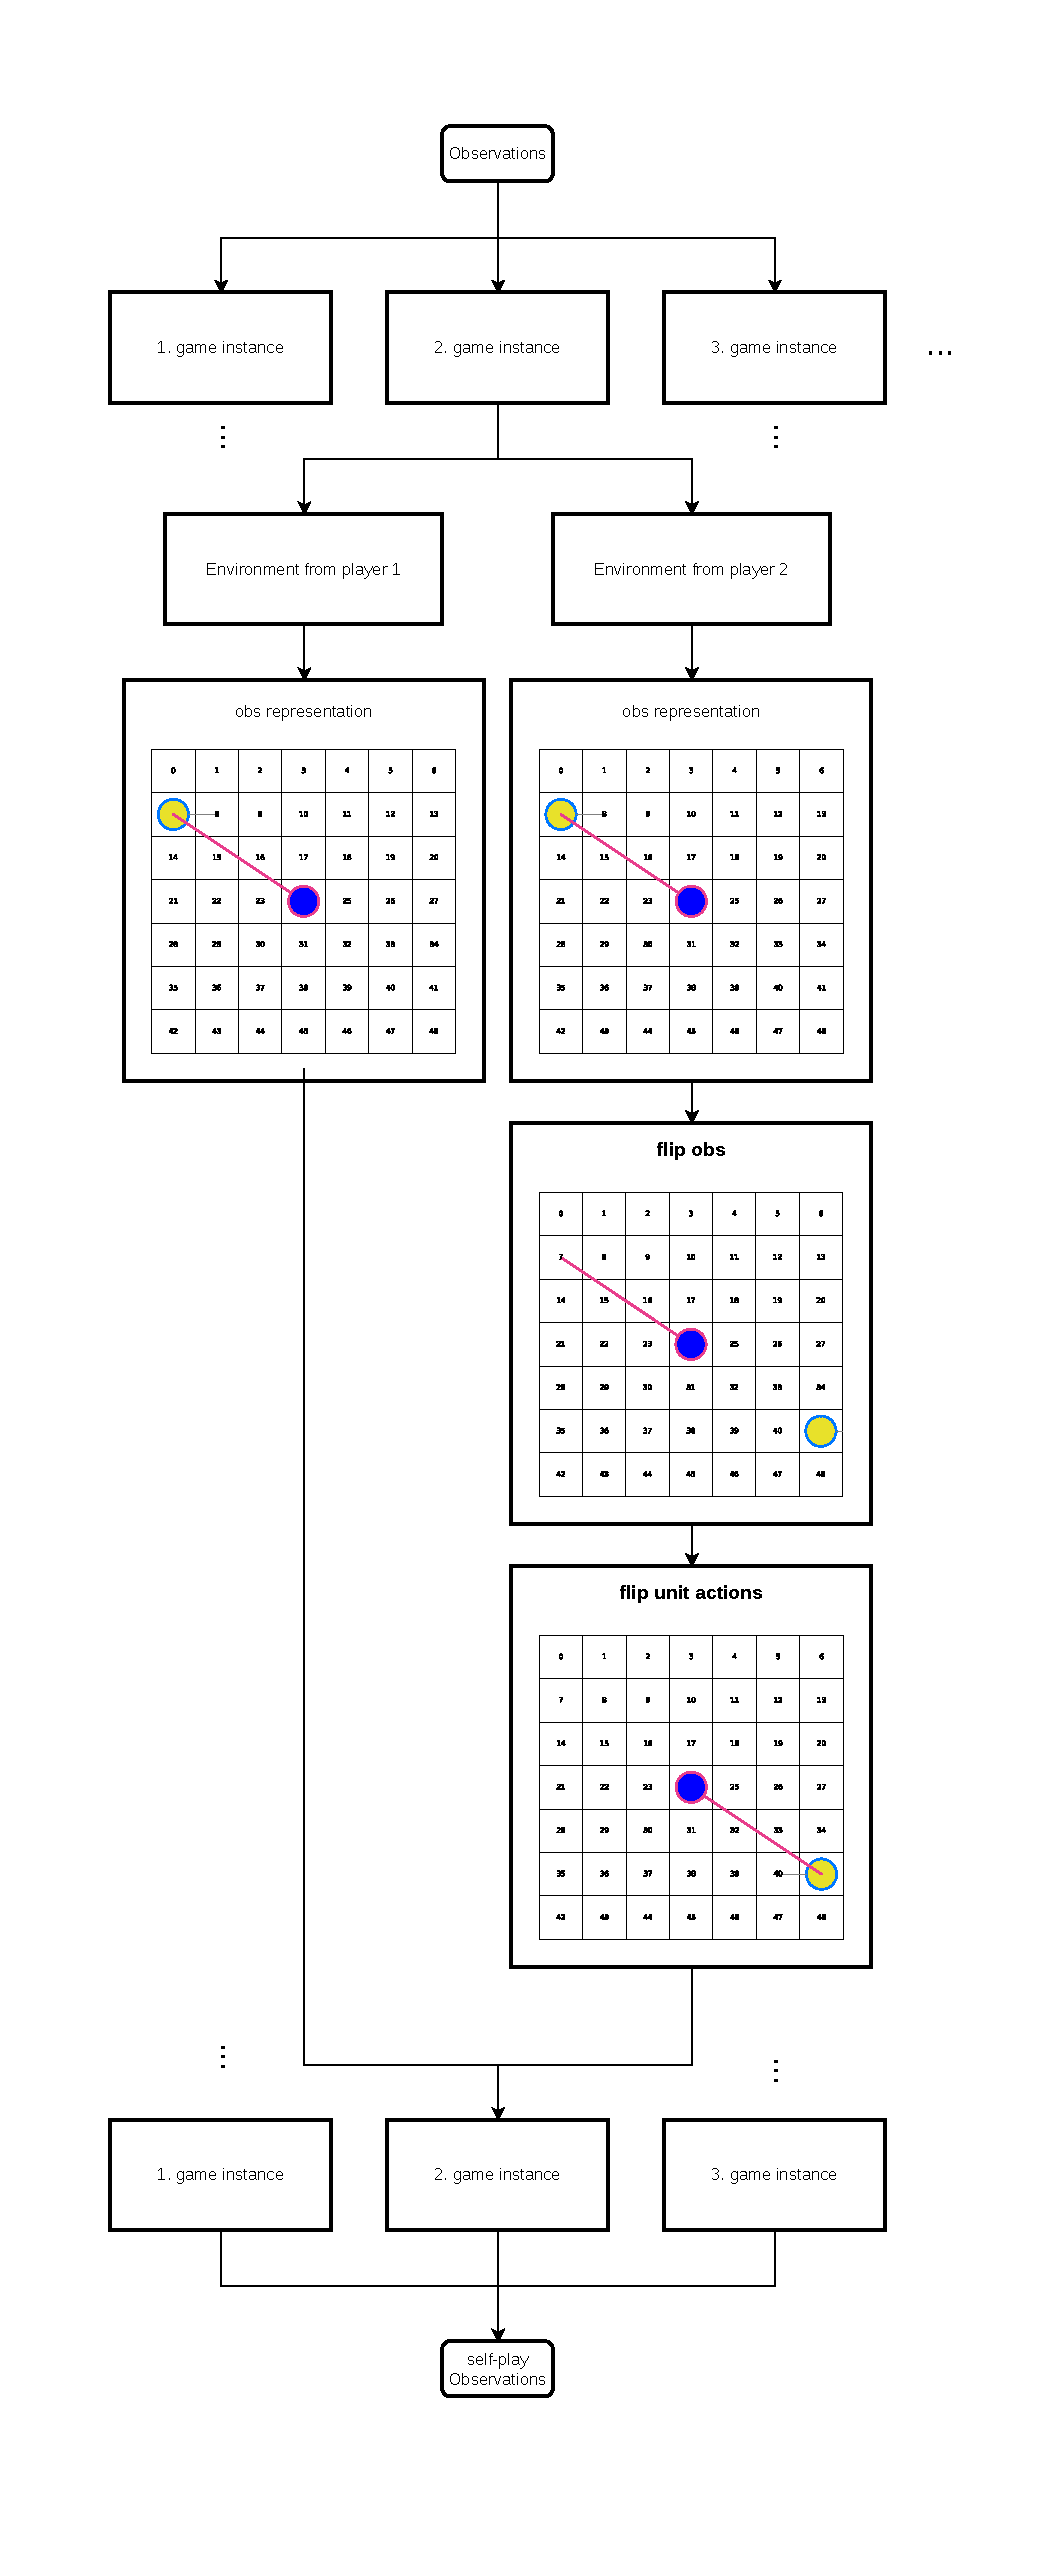
\includegraphics[width=\linewidth,height=1\textheight,keepaspectratio]{images/adjust_obs.pdf}
    \captionof{figure}{Observation adjustment for player 2 in SP.
    To rotate the observations, the GridNet representation was flipped for each player-2 environment.
    The unit actions in the observation were then flipped individually.}
    \label{fig:adjust_obs}
\end{center}
Actions are transformed accordingly, so that the environment still executes the intended actions for player 2.
Masks must be transformed as well, since they are based on the environment’s observations.
The same rotation used for the observations is also applied to the invalid action masks. 
After masking, the selected actions (including a position component, that is added before masking, since masking removes the implicit positional structure of the GridNet action space) are transformed back to fit the MicroRTS-Py environment.


\subsection{fictitious self-play (FSP)}
To address the instabilities of pure SP, in FSP the agent is trained not exclusively against the current policy, but against a uniformly sampled pool of the agent’s historical policies. 
This results in the learning agent learning a good response to the averaged opponent strategy, which reduces cyclical learning.
Under standard assumptions, FSP can converge towards an approximate Nash equilibrium in two-player zero-sum games (with respect to the average strategies).
Heinrich et al. also demonstrate this empirically in poker experiments \cite{heinrich2015fsp}.

\paragraph{Implementation.} 
The implementation is similar to SP, but instead of Player 2 always using the current policy, Player 2 is sampled uniformly from a pool of historical agents (snapshots of the Main Agent at different training stages).

\paragraph{Problem with the implementation.} 
If we implement in the described way, a problem arises: player 1 has priority in conflict resolution (e.g. when both players want to move to the same cell).
This gives player 2 a disadvantage, although it has only a minor effect on the results. 
The actual problem is that the agent can exploit this prioritization in FSP if it learns that optimizing the training objective can be achieved primarily by improving player 1, while deliberately performing poorly as player 2.
After sufficient training, the agent will learn a strategy that is based on player 1 being prioritized.
Training then stagnates, since the agent already has a hight winrate against itself without develping a robust strategy against other opponents.

\paragraph{Example.} 
The agent could learn to block an opponent in front of the Base by issuing a simultaneous move to the same target cell.
In FSP, player 2 would then be blocked, while player 1 would not, allowing the agent to achieve a win rate close to 100\% against itself.

\paragraph{Relevance for LT.} 
In LT, the Result of the problem is not quite as problematic because there are exploiters that can be trained against, which remain adversarial to the Main Agent.
However, a large portion of the training becomes ineffective and provides poor learning signals if the agent exploits the player 1 priority.
On top of that the Problem is particularly relevant for LT, which combines SP and FSP, because only historical Agents are available for training in FSP, making the feedback for player 2 very sparse, while in LT the Main Agent can directly train against the current Main Agent.
This yieldes more immediate feedback on  the Main Agents performance as an opponent (player 2).
As a result the agent no longer has to plan as far ahead in order to exploit this priority and minimize its own win rate as player 2.
\begin{figure}[h]
    \centering
    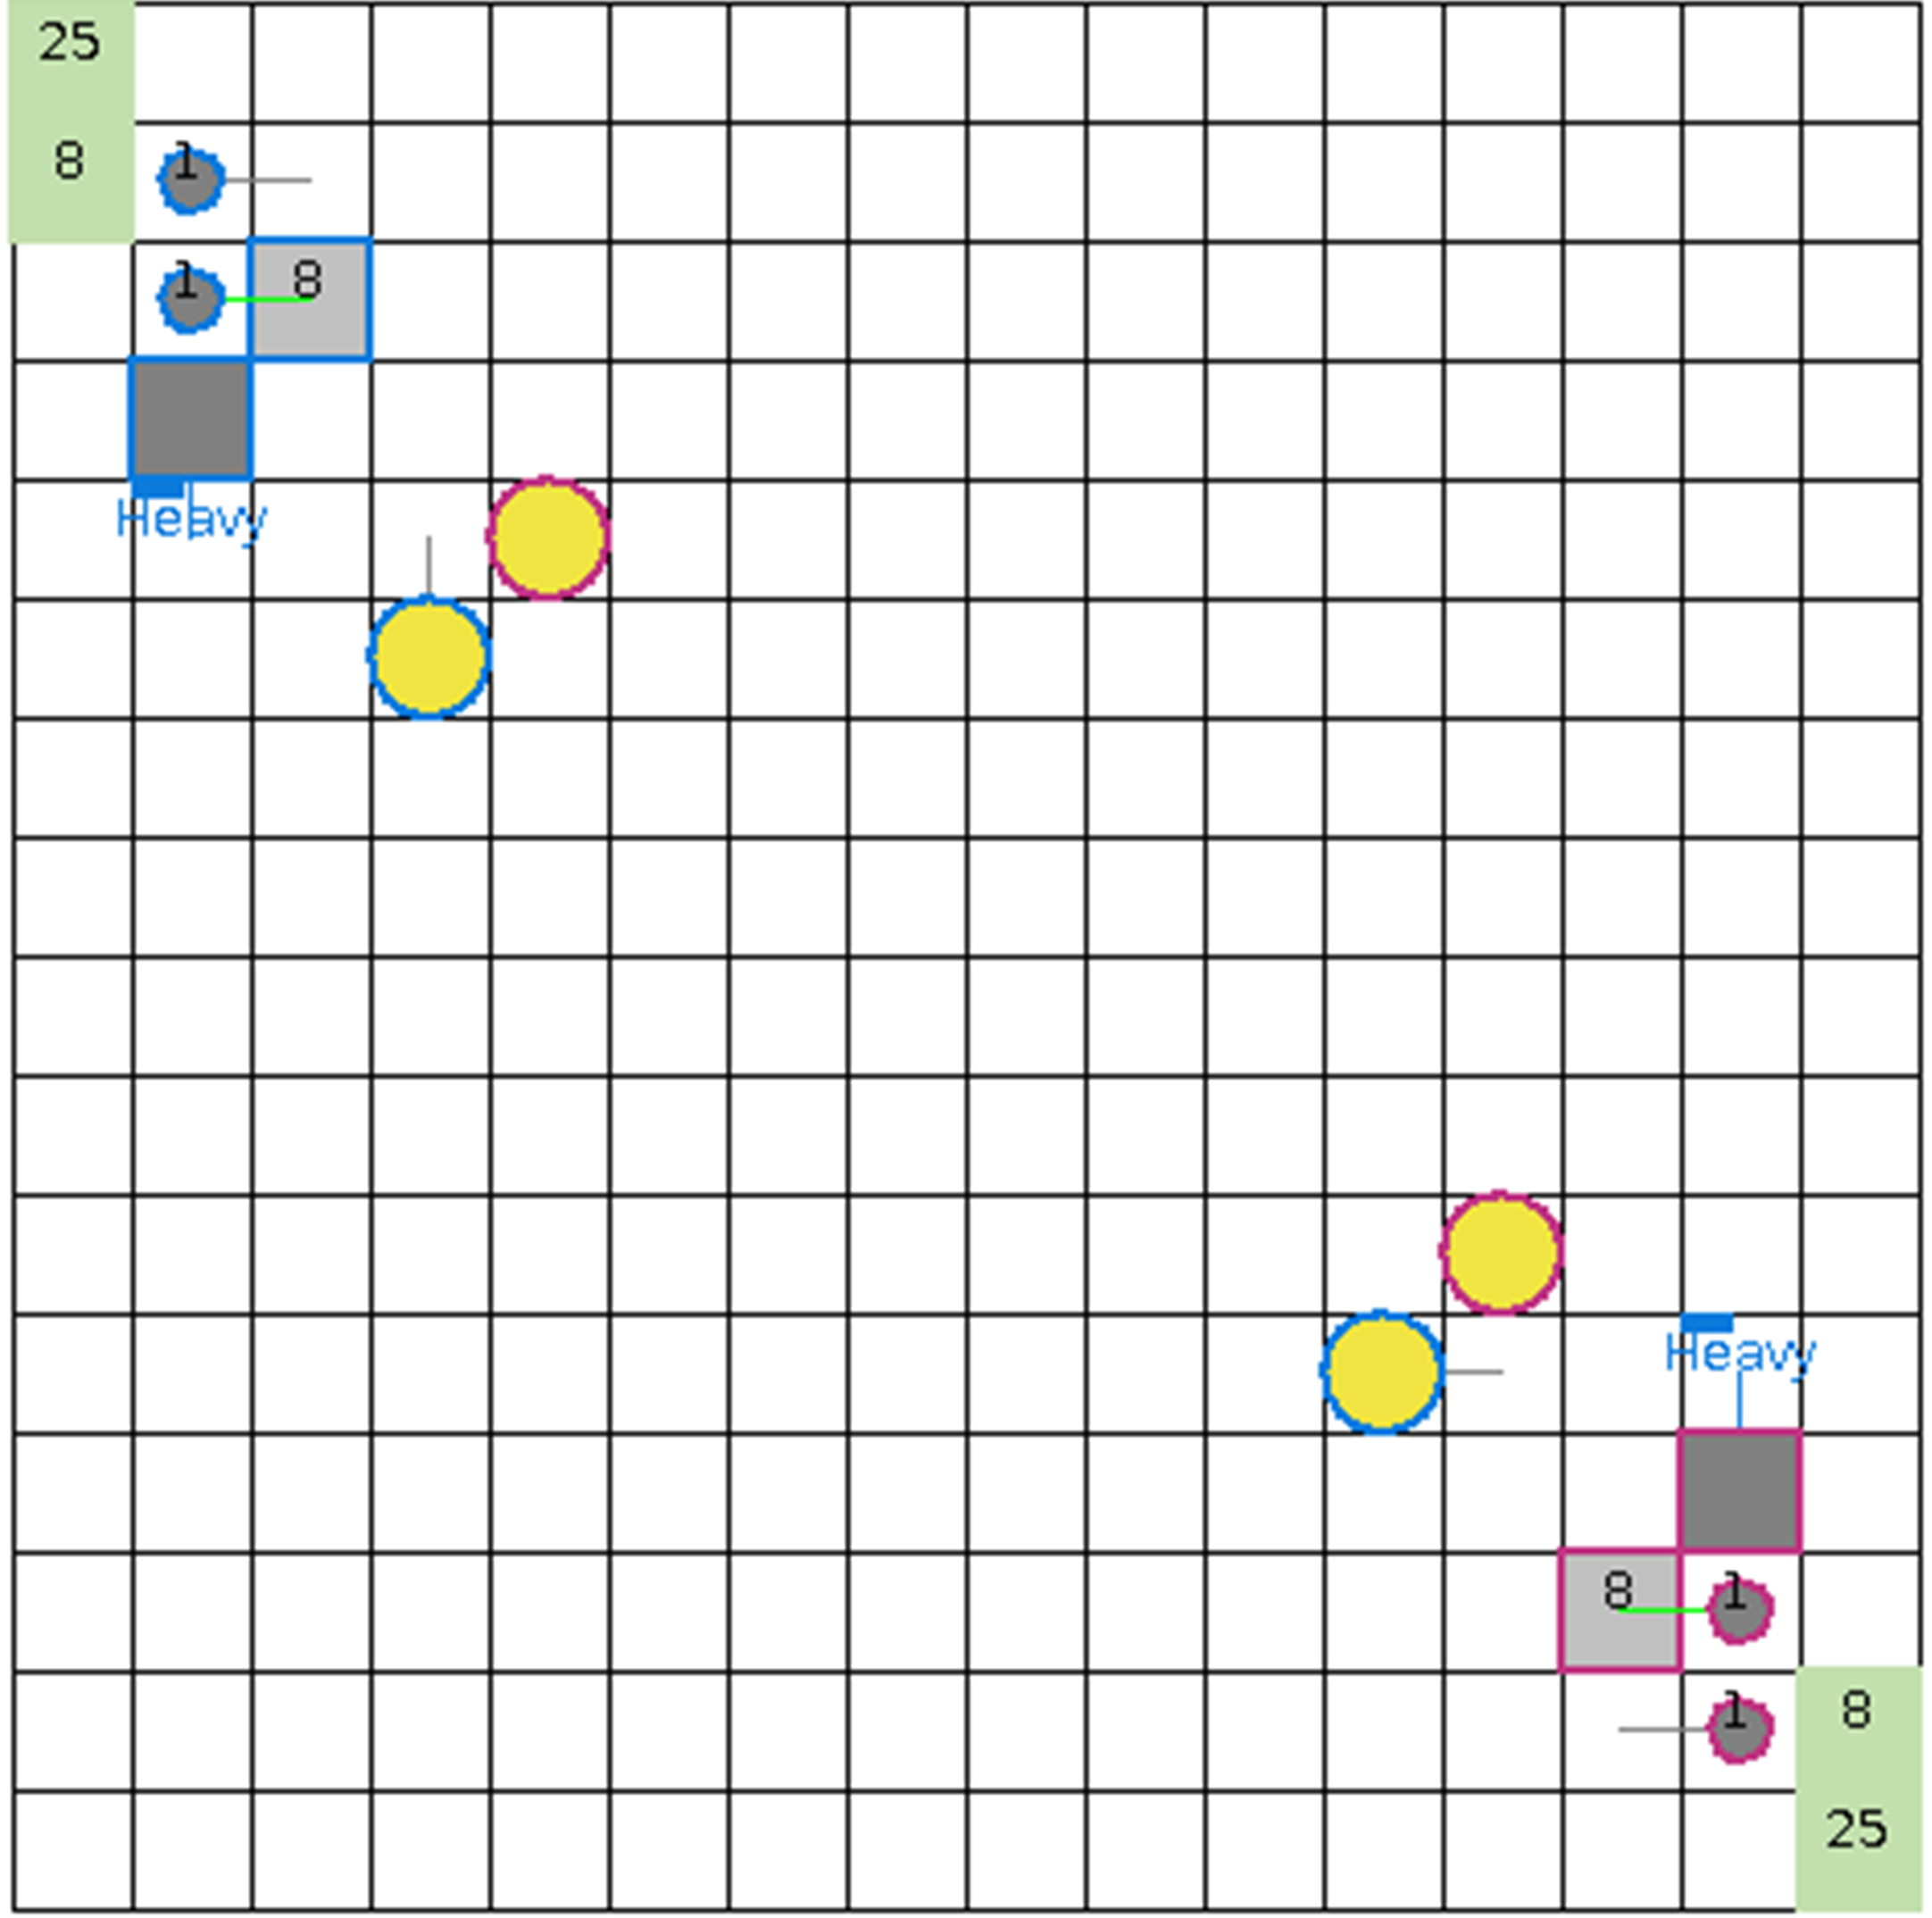
\includegraphics[width=1\linewidth]{images/action_konflikt.png}
    \caption{Screenshot showing an action conflict in the game.
    Both Heavy units of both players wanted to move to the same cell, as the opponent’s Heavy units.}
    \label{Figure 3}
\end{figure}

\paragraph{Solutions.}
In the re-implementation of MicroRTS-Py, there is a mode that resolves conflicts in a randomized manner.
However, this does not help in this case, because even before the conflict arises, invalid action masking masks out the action of player 2 since it is invalid.
To solve this problem, the learning agents in the parallel games are alternated between playing as player 1 and player 2.
This does not prevent the prioritization of player 1. 
However, it can be shown empirically that the prioritization of player 1 has no major impact on the results.
% TODO: füge ein Ergebnis ein, in dem die Ergebnisse von 2 gegeneinander spielenden Agenten 1 mal als Spieler 1, 1 mal als Spieler 2 dargestellt werden.
% Evaluation vs 22_02_2026__finished_PPO_Basis_thesis__args_working_main_5_3_4_update_1986 over 200 games | win: 76 (38.00%), draw: 56 (28.00%), loss: 68 (34.00%), avg reward: 1.403
This prevents the exploitation of the prioritization by the learning agent, since it can now also be player 2 and therefore a strategy that is only effective for player 1 is no longer beneficial.


\subsection{prioritized fictitious self-play (PFSP)}
LT uses an extended variant of FSP called PFSP \cite{vinyals2019alphastar}.
PFSP extends FSP by selecting opponents against which the agent can train efficiently, rather than selecting opponents uniformly.
The selection probability is based on the win rate of the learning agent against the potential opponent \cite{vinyals2019alphastar}. 

\paragraph{Prioritization Function.} 
The exact prioritization function can differ for different agent types.
In AlphaStar, for the Main Agent, opponents of medium difficulty (win rate close to 50\%) are prioritized. While exploiters prioritize the strongest opponent (against which the win rate is closest to 0\%).
Adapted prioritization functions tailored to our training setup are used in this thesis,  which deviate from those used in AlphaStar.
An important difference is that training against an opponent against which the base agent has a win rate close to 0\% yields little informative gradient or learning signal.
% und dass eine win rate von 0.5 meist heißt, dass keiner von beiden gewinnt/verliert. 
% Stattdessen hieß das meistens, dass beide Spieler sich gegenseitig ignorieren, die Basis des Gegners angreifen und dann für den Rest des Spieles sich nicht mehr bewegen.
% Durch diese Spielsituation verlangsammt sich das Training, deshalb werden in dieser Arbeit Gegner mit einer win rate die kleiner als 0.5 ist mehr priorisiert als 0.5.

\paragraph{Implemented Prioritization Function.} 
To avoid opponents resulting in little learning signals, the following prioritization functions was used for the Exploiters:
\begin{center}
    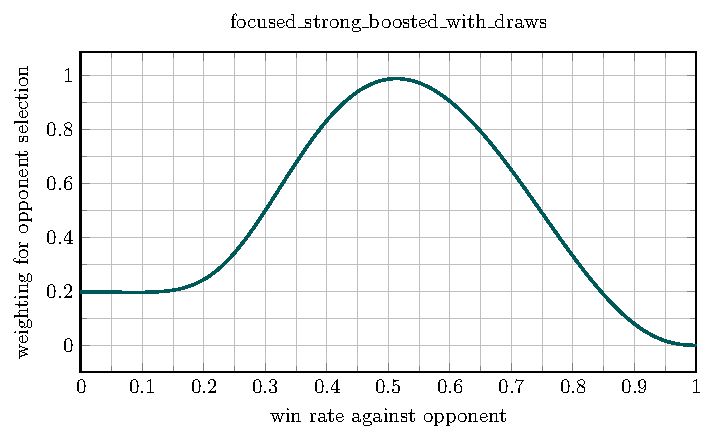
\includegraphics[width=\linewidth,height=1\textheight,keepaspectratio]{images/focused_strong_boosted_with_draws.pdf}
    \captionof{figure}{Prioritization function for the Exploiters in PFSP.}
    \label{fig:focused_strong_boosted_with_draws}
\end{center}
As can be seen in the figure, we prioritize opponents with a low win rate not close to 0\%. Furthermore, opponents with a win rate of 0\% are prioritized over those with a win rate of 100\%, since there is substantial learning potential for an opponent with a win rate of 0\%, whereas a win rate of 100\% usually means that the agent already defeats the opponent reliably.
In this thesis PFSP was modified so that all agents have a non-zero probability of being selected. This ensures that no opponent is completely ignored because it lost all initial games (yielding a 100\% win rate for the learning agent), since these initial results may have been outliers.


% Das wurde so umgesetzt: probs = (1.0 - min_prob_factor) * probs + min_prob_factor * uniform



% Bild einfügen?

\subsection{league training (LT)}
\label{sec:LT}
LT combines and extends SP and PFSP to further stabilize training.
It also promotes robustness by training against opponents sampled from a \emph{league}, including Main Exploiters and League Exploiters and Historical Agents \cite{vinyals2019alphastar}.

\paragraph{League composition and roles.} 
Learning Agents of the league were trained in parallel.
Similar to AlphaStar \cite{vinyals2019alphastar}, the league in this thesis consists of the following agent types:
\begin{itemize}
    \item \textbf{Main Agent (MA):} The primary policy that is optimized and evaluated.
    \item \textbf{Historical Agents:} Frozen snapshots of earlier MA or exploiter agent policies. 
    They stabilize training by providing a distribution of past strategies and mitigate catastrophic forgetting.
    \item \textbf{Main Exploiters (ME):} Agents trained only against Historical Main Agents, which encourages them to identify and exploit weaknesses in the Main Agent.
    \item \textbf{League Exploiters (LE):} Agents trained against all Historical Agents, which further promotes diversity by identifying systemic weaknesses of the league.
\end{itemize}
Historical Agents are the only agent type that is not a learning agent.
The main differences between the roles are the opponent-sampling distribution and the hyperparameters.
All agents share the same observation/action representation (GridNet with invalid action masking) and use the same underlying PPO algorithm, but are trained with role-specific hyperparameters (e.g., learning rate and PFSP prioritization function).


\paragraph{Training loop and snapshot management.}
LT iterates through cycles consisting of the following phases:
\begin{enumerate}
    \item \textbf{Select opponent:} Sample an opponent from the league.
    \item \textbf{Collect rollouts:} Run matches between the learning agent and the sampled opponent for a fixed number of steps. No agent is updated during this phase.
    \item \textbf{Update policy:} Perform PPO updates using the collected trajectories against the sampled opponent.
    \item \textbf{Update statistics:} Periodically evaluate against a subset of league members to update win-rate estimates used by PFSP.
    \item \textbf{Add snapshots:} At predefined intervals (or when performance criteria are met), store a frozen copy of the current agent as a new Historical Agent.
\end{enumerate}
A phase of the training loop is considered completed only after every agent type (MA, ME, LE) has completed the phase.
For example, the Main Agent only proceeds to the next phase after all Main Exploiters and League Exploiters have completed the current phase.

\paragraph{Bot environments.} 
Bot environments are added to the league to stabilize training by continuing the PPO training against the built-in MicroRTS bots CoacAI and Mayari, which the base agent was trained against.
Only the Main Agent trains against the built-in bots, since learning signals from built-in bots could interfere with identifying and exploiting weaknesses in the Main Agent or the league, which is the main purpose of the exploiters (e.g., if the built-in bots are too strong against an exploit that the Main Agent has not yet trained against).
In MicroRTS-Py the environments for built-in bots and for SP are not interchangeable, since the built-in bots are not implemented as neural policies and therefore cannot be used in SP/FSP/LT directly. 
The number of parallel environment instances and their built-in bot opponent (if any) have to be defined at initialization of the MicroRTS-Py environments, which means the number of environments for each built-in bot remains fixed.
One of the main advantages of LT is that training against opponents with bad learning signals is reduced.
To retain that improvement we want the number of bot environments to be dynamic.
Therefore, the number of bot environments is adjusted dynamically by reinitializing a MicroRTS instance, which is only used for training against the built-in bots and not for SP/FSP/LT (because reinitialization also means resetting the environments in the MicroRTS instance).
The MicroRTS instance for built-in bots executes its step function at the same time as the SP/FSP/LT instance.

\paragraph{number of parallel bot environment instances.}
Two hyperparameters define the maximum number of parallel bot environment instances and the minimum number of parallel bot environment instances.
% TODO: A Buffer for observations, actions, invalid action masks with ... % zu viel Codedetails?
Among other things, references to the observation, action, and invalid action mask buffers must be adjusted to the correct size and partially reset whenever the number of parallel bot environment instances is changed.
% TODO: alle "invalid action mask" zu "invalid-action-mask"?


\paragraph{Summary: Opponent Selection.}
PFSP samples the next opponent from a given set of possible opponents, with probabilities based on the current learning agent’s win rates against the potential opponents, whereas SP always trains against the current learning Agent.
The opponent selection for the League is illustrated in Figure \ref{fig:Matchmaking}.
Depending on the agent role, opponents are either the current Main Agent or sampled from specific subsets of historical agents using PFSP. 
The Main Agent also trains against additional bot environments, while Main Exploiters and League Exploiters are matched only against agents from the league.
% TODO: vielleicht die Grafik erst ans Ende verschieben und hier nur verlinken. Dort dann über die Gesammte Seite.
\begin{center}
    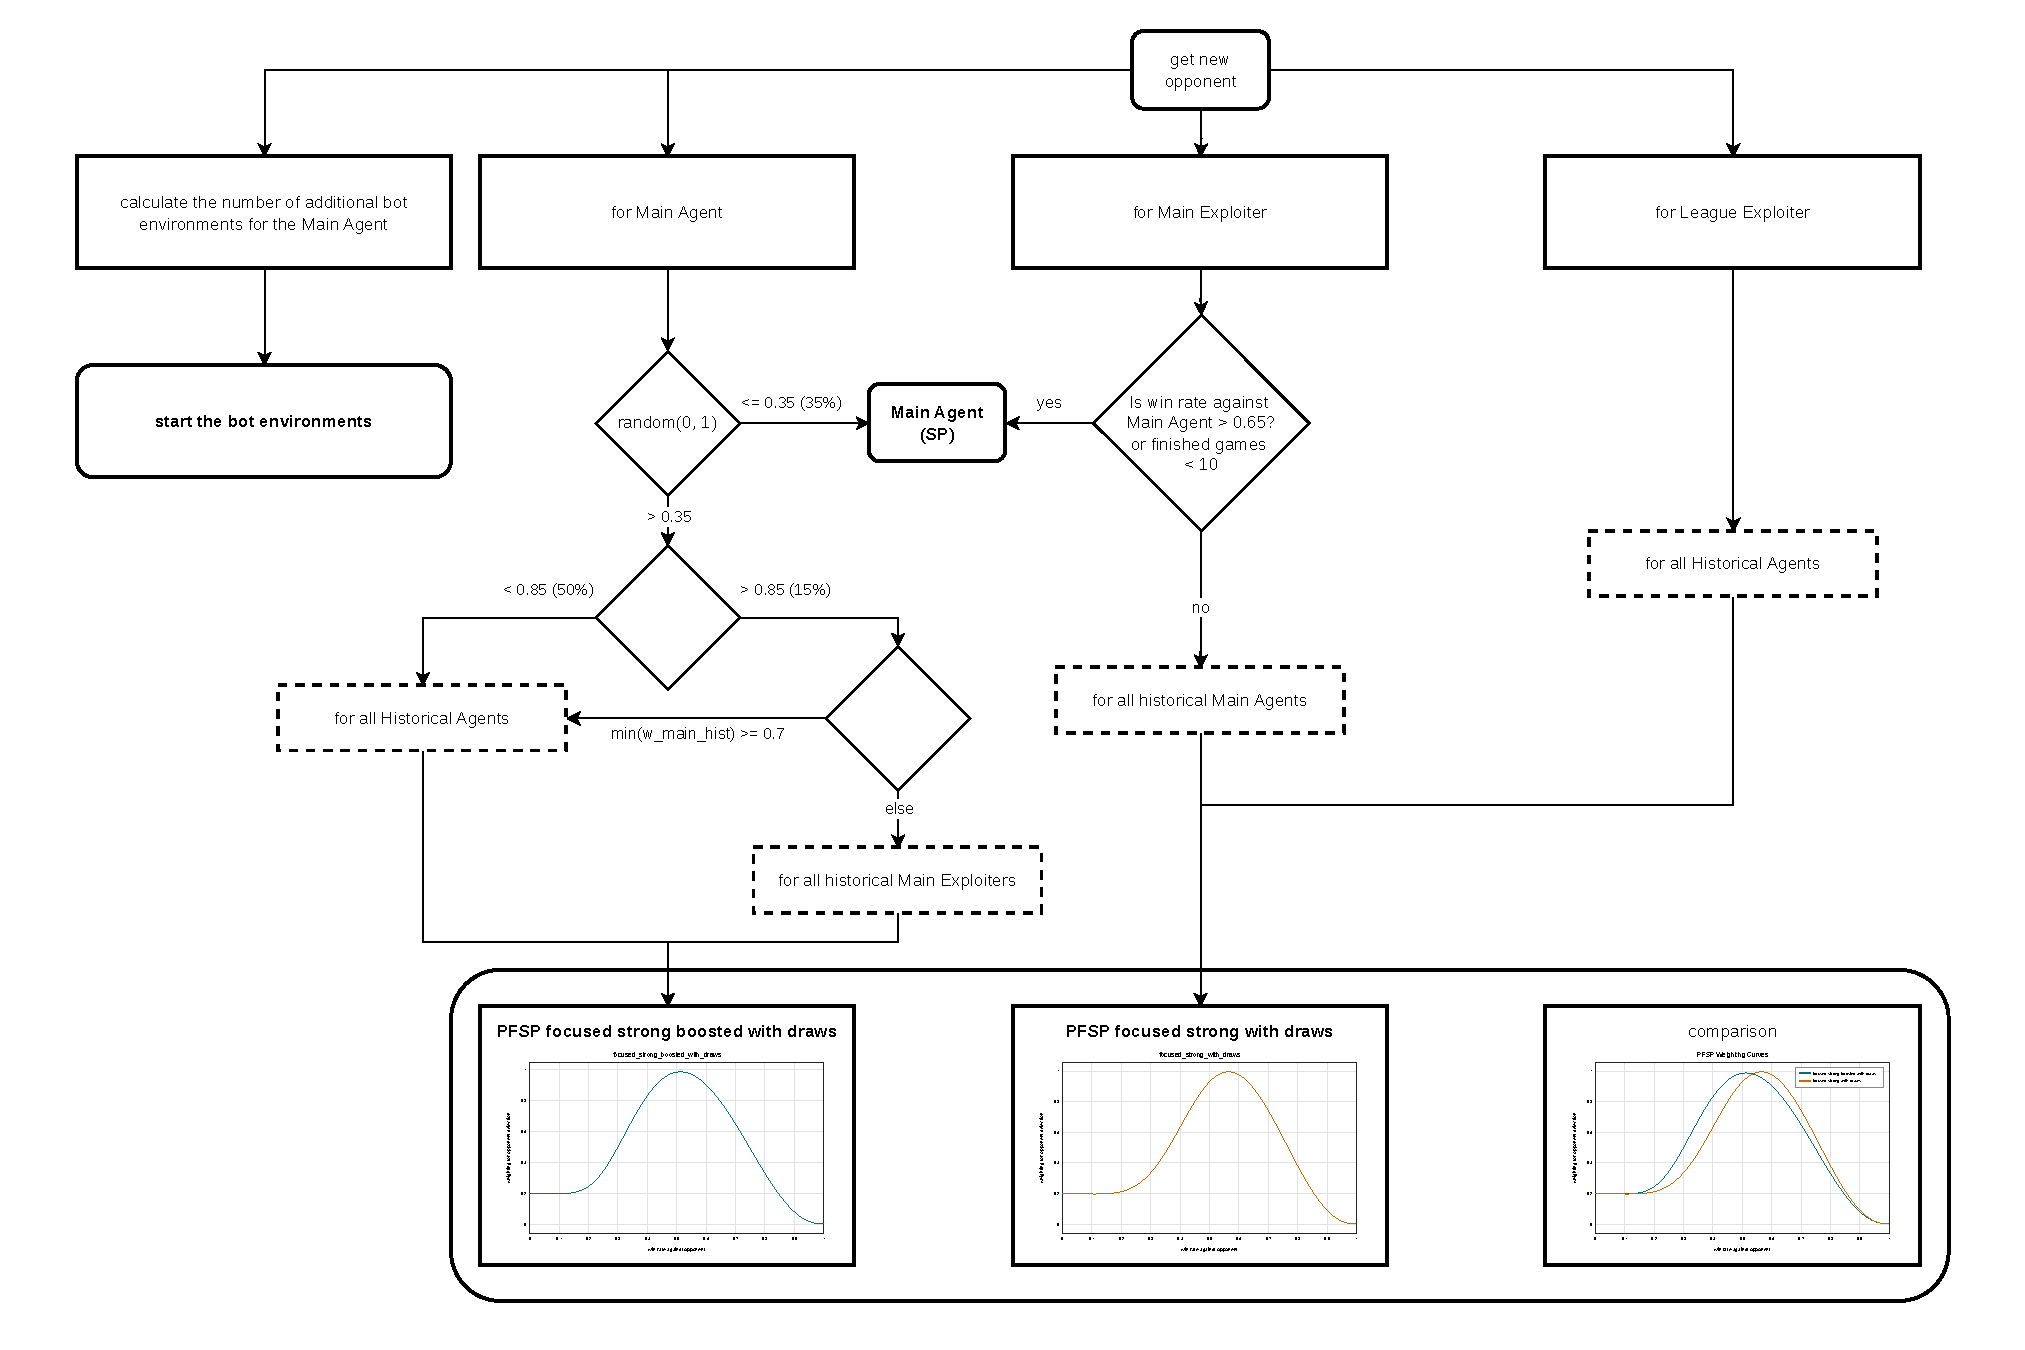
\includegraphics[width=1.2\linewidth, height=0.5\textheight,keepaspectratio]{images/Matchmaking.pdf}
    \captionof{figure}{Matchmaking process for the league. Dashed boxes are candidate opponent sets, while the percentages on the arrows are fixed sampling probabilities. The PFSP curve gives the weighting for the opponent win rate}
    \label{fig:Matchmaking}
\end{center}

% TODO: ab hier überarbeiten
\paragraph{Resetting Exploiters.}
% TODO: unit bonus distribution im Text lassen?
The Paper for AlphaStar \cite{vinyals2019alphastar} only explains that exploiters reset their weights however, in this theses exploiter resets also reset optimizers, game statistics (e.g., win rates so that PFSP does not use outdated information) and the unit bonus distribution (if applicable).
On top of that exploiters only reset after the game ended, which means exploiters can reset in an rollout.
If that happens, then the rollout contains trajectories from the old policy and therefore can not be used for the on-policy training.
To keep the training as simple as possible, the entire update after an exploiter reset is skipped.



\paragraph{Alphastar Pseudo Code.}
In addition to the modifications to fit the Pseudo Code to the new Environment the following corrections to the pseudocode for AlphaStar in the original paper \cite{vinyals2019alphastar} where made:
\begin{itemize}
    \item While resetting Exploiters the pseudo code first reset the weights and then saved the snapshot for the Historical Agent, now the order is reversed, so that the snapshot is not of the reset Exploiter.
    \item Main Exploiters where only trained against the current Main, if it has a high winrate against the Main Agent from the very start.
    As soon as the win rate against the Main Agent dropped the Main Exploiter stopped training against the Main Agent for the rest of this reset cycle.
    However in the pseudo code Main Exploiters only reset/checkpointed (which creates a Historical Main Exploiter), if the win rate against the Main Agent is high, which means that the Main Exploiter would never reset if it initialy had a low win rate against the Main Agent.
    Since the current Main Exploiter has already trained against the Base Agent, it is very likely that the Main Exploiter never checkpoints before the maximum number of steps is reached, even if it has a high win rate against the all historical Main Agents.
    To solve this Problem the win rate against the Main Agent is replaced with the minimum win rate against all historical Main Agents.
    This ensures, that the Main Exploiter is reset and checkpointed as soon it is likely achieving a high win rate against the Main Agent and does not have much to learn from the possible opponents.
    \item Another change to the pseudo code is that the win rates are set to 0.5 for the initial games, which makes it less likely that the agent will ignore opponents that it has not yet played against, which could be outliers with a very high or low win rate, including the Main Exploiter and Main Agent matchup.
\end{itemize}





\subsection{Additional modifications for diversity}
The Biggest problem with the training setup is the opponent diversity.
To make exploiters more diverse the exploration can be increased with hyperparameters such as learning rate and entropy coefficient and kl regularization coefficient.

\paragraph{Problems with overall increased exploration.}
Excessively increasing the exploration for exploiters can lead to worse performance and longer training.
We Hypothesis that the problem is that the starting point (the Base Agent) is already very strong and the effective strategies for different unit types are very different, which means that the agent has to almost entirely unlearn the current strategy, before it can learn new strategies for other units.
In between the unlearning and learning phase, the agent performs very poorly, which leads us to belive there are very distant clusters (corresponding to different unit types) of local maxima in the reward landscape, which is why finding different maxima with the same unit type is possible, but changing to a strategie for different unit types very difficult and time-consuming.
Furthermore, the same problem occurs for every exploiter, multiplying the problem.
What makes diversity even more difficult is that in a complex environment such as MicroRTS, league training will most likely not cover all possible Main Agent weaknesses, that can be exploited by an exploiter using Heavy Units (which the Base Agent strongly favors).
This means that we expect, that there are always easier to reach weaknesses than weaknesses exploitable by changing the focused Unit, even after the training.
% TODO: Beispiel behalten?
For example if the Base Agent that favors an attack using Heavy units is to exploit a weakness, that occurs when the Main Agent is attacked by many Worker units, then for every step every Worker on the field is not allowed to build Barracks (which wastes too many Recources to make the strategy work).
Instead of using only 2 Workers the Agent has to produce as many as possible and but two units have to rush the opponent.
The Agent only gets rewarded positively, if all of that happens in the same game, making it unlikely to occur.
The second strategy in the example is a built-in Bot strategy of MicroRTS called workerRushAI.

\paragraph{Producing Exploration Bonus.}
To further increase Exploration, without decreasing efficiency too much, an exploration bonus targeting the production of Workers, Ranged, Heavy and Light Units can be added to the reward.
By targeting the production of different Units, the agent is encouraged to explore different strategies for different Units, which can lead to more diverse exploiters.
This was achieved, by using a mask, to only give Barracks and Bases (which can only produce Units) a bonus for Entropie.
While  this helped to increase Exploration with other units, which can be seen because the Agent uses more different Units, it was not enough to make the agent explore different strategies for different Units.
% TODO: Bild von Unit Count nach Spiel ende mit und ohne Bonus?

\paragraph{Unit Bonus.}
To address the problem of insufficient diversity, a clipped unit bonus can be added to the reward, encouraging the agent to use different units (e.g., by giving the Base Agent a bonus every time it produces a Ranged Unit).
The number of other Units increased, while using the Unit Bonus, however even with weaker Agents like the agent state after the BC phase and over 20 Million steps, the agent did not use strategys for different units and instead produced the Units with an Bonus at the End of an Round, when the result was decided.

\paragraph{Unit Bonus Distribution.}
Unit Bonus Distribution is an improved methode to increase the diversity of exploiters based on the Unit Bonus.
The Idea is to continue training the Agent with a new feature, that recieves a the Unit Bonus, that is sampled from a distribution which is updated every game.
Then the trained Agent can be used as an Exploiter with an static bonus/distribution bonus, resulting in an Exploiter with definable tendencys toward different Units.
This also allows to retrain the BC and PPO phases with the Unit Bonus, because only 1 Agent needs to be trained instead of multiple with different fixed Unit Bonus, which would be very time consuming.
% TODO: entfernen? Bild? Run?
Retraining the Agent from scratch with the Unit Bonus Distribution showed promising results, however the training was not continued long enough to evaluate the effect of the Unit Bonus Distribution on the diversity of the exploiters, since the training with the Unit Bonus Distribution is very time consuming, because the BC phase did not work with the Unit Bonus Distribution methode and had to be skipped.
Continuing the Trainig with the Basis Agent had the same problem as the training with the Unit Bonus.
% \subsection{Neural Network Architecture}






\label{sec:nn-architecture}

 





\section{Experimente}
\label{sec:experimente}

% \subsection{Setup}
\begin{table}[h]
\centering
\caption{Training parameters for PPO training.}
\begin{tabular}{l c}
\hline
\textbf{Parameter} & \textbf{Value} \\
\hline
Initial learning rate (Adam) & $2.5 \times 10^{-5}$ \\
Rollout steps per environment & 512 \\
Minibatch Size & 3072\\
Max episode length & 2,000 timesteps \\
Discount factor $\gamma$ &  1 \\
Value function coefficient $\beta$ & 0.01 \\
Entropy coefficient $\eta$ & 0.005 \\
Gradient norm threshold $\omega$ &0.5 \\
KL regularization coefficient $\lambda_{\text{KL}}$ & 0.4 \\
GAE parameter $\lambda$ & 0.95 \\
\hline
\end{tabular}
\label{tab:training_params}
\end{table} 

% \subsection{Results}




% \subsection{Discussion}




\section{Conclusion}
\label{sec:conclusion}



% \section{Reproducibility and Codebase}




%%%%%%%%% REFERENCES
{\small
\bibliographystyle{apalike}
\bibliography{references}
}

%%%%%%%%% Erkl\"arung
\onecolumn
\pagebreak\noindent
\textbf{\LARGE Erkl\"arung}
\addcontentsline{toc}{section}{Erkl\"arung}

\bigskip\bigskip
\noindent 
GPT!!!!!!!!!!!!!!!!!!!!!!!!!!!!!!!!!!!!!!!!!!!!!!!!!!!!!!!!!!!!!!!!!!!!!!!!!!!!!!!!!!!!!!!!!!!!!!!!!!!!!!
Hiermit versichere ich, dass ich die   Bachelorarbeit selbst\"andig verfasst und keine
anderen als die angegebenen Quellen und Hilfsmittel benutzt habe.

\bigskip
\noindent
D\"usseldorf, den XXXXXXXXXXX

\bigskip\bigskip\bigskip
\noindent
{Name!!!!!!!!!!!!!!!!!!!!!!!!!!!!!!!!!!!!!!!!!!!!!!!!!!!!!!!!!!!!!!!!!!!!!!!!!!!!!!}

\newpage

\end{document}
